\section{Introduction}

A business rule articulates some aspect of the expected functional behavior (or a \textit{requirement})
of an enterprise application. Here is a simple business rule that determines how an invoice total is 
determined in a billing application:

\begin{quote}
	The \textit{Balance Type} of a customer affects how invoice total is computed; it can be 
	one of the following:

	\textit{None}: The customer's account will not hold a balance; instead all charges accrued 
	in an order will be included in the next invoice;
	
	\textit{Credit}: The customer's account may accrue charges up to the set credit limit. 
	Charges will automatically be paid from the users credit pool until the set limit is reached. 
	Users are responsible for paying their credit debt as well as any overages.
\end{quote}	

We will examine this rule closely later; for now, suffice it to say that the requirements 
of an enterprise system are typically captured by a large number (often in hundreds) of business rules
such as the one above.

It is reasonable to expect functional testing of an enterprise system to \textit{cover} its 
business rules, which is to say, testing would exercise every distinct scenario described in each of
its business rules.  For example, in the above rule, one of the specific scenario to be exercised is
that a customer's balance type is credit, and that the order amount does not exceed the credit limit.
A test that exercise this scenario would set up a customer with the balance type as credit as a certain
credit limit, create an order with the appropriate constraint on the order total, and then finally
create an invoice for that customer, and verify the invoiced amount.  (See Figure~\ref{fig:jbilling-flow}) Thus, it requires a carefully 
thought out test scenario (i.e. a sequence of test steps) as well as associated test data to exercise 
a business rule, or a scenario thereof.

\begin{figure*}[t]
\centering
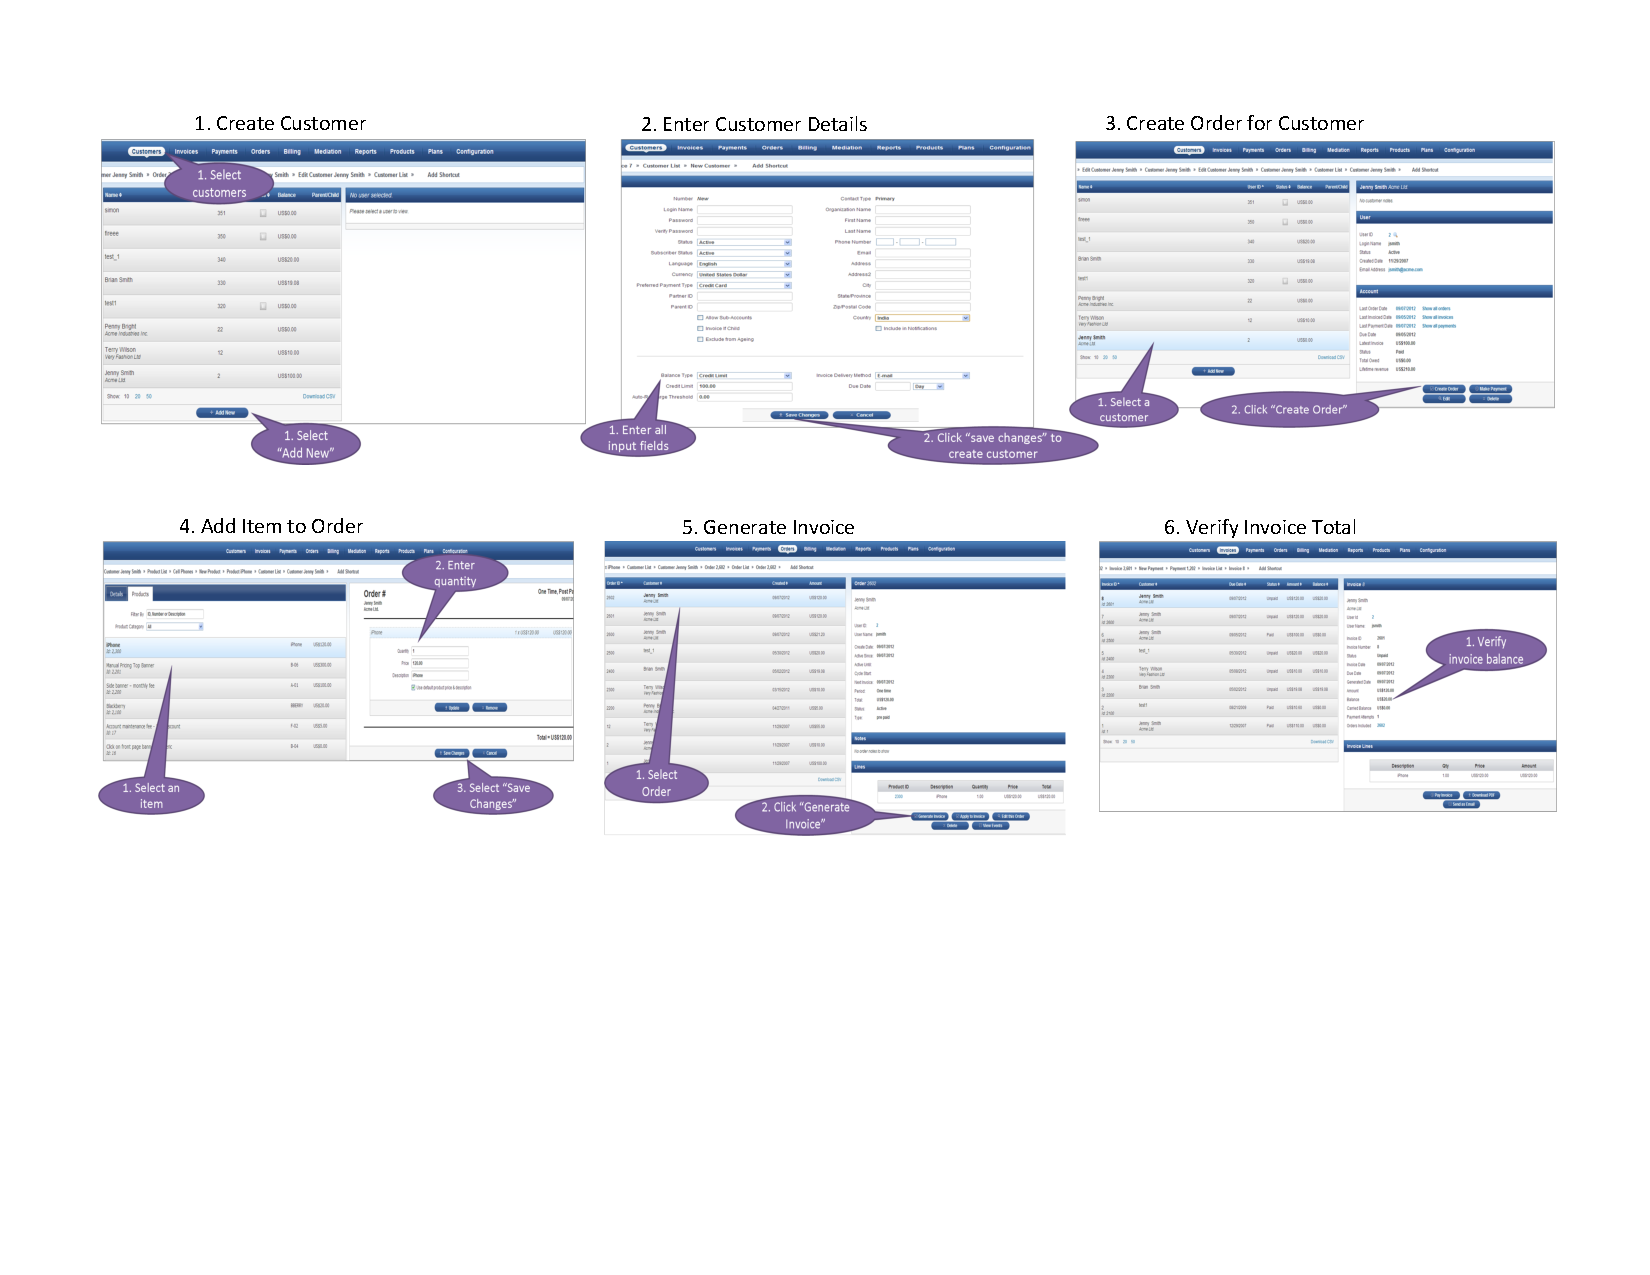
\includegraphics[width=7.5in]{figs/jbilling-flow}
\caption{Test sequence for a JBilling business rule}
\label{fig:jbilling-flow}
\end{figure*}

In practice, due to time pressures, testers are more often ad hoc than methodical in creating test 
scenarios and test data.  One part of the problem is that in realistic system might have hundreds of 
business rules written out in plain text, and it is difficult to grasp a global view of how the rules 
together describe the application behavior.  A related part of the problem is that it needs complex 
reasoning to piece together test sequences that would cover each scenario. Consequently, testers may 
create tests that exercise the same business rule, or a scenario thereof, repeatedly without additional 
benefit in quality assurance, and more problematically, may neglect to create tests for some other business 
rules.  The net result of this state of affairs is that despite a lot of resources spent in testing, bugs 
still escape into the field.

Our vision is to advance the state of the practice in testing of enterprise software by making it more
tool based, by adapting technology developed for automated and systematic test generation for programs.  
In this vision, business rules would be written in a structured notation that allows mechanized analysis. 
(Special editors could be created to enable non-programmers to capture business rules in a structured notation; 
this is an independent challenge in \textit{end user} programming).  A tool would validate business rules 
and point out any ambiguities or omissions that it can detect.  After the business rules pass validation, 
another tool would generate test sequences and test data to exercise the application thoroughly as well as
without redundancies.

%Randomly generated test data cannot be expected to suffice for enterprise
%applications with complex rules. Also, systematic test-generation approaches
%based on program analysis (\eg \cite{Emmi:2007,Li:2010,Marcozzi:2012,Pan:2011})
%cannot be expected to tackle enterprise applications, which use a mix of
%multiple language and database technologies in their implementation. Moreover,
%these techniques are directed toward attaining simple forms of code coverage,
%such as statement or branch coverage, rather than coverage of complex business
%rules.

At first blush, this problem seems to be similar to the problem of testing
programs written as control-flow graphs, with the goal of exercising each acyclic path in the 
program.  The problem is different from path coverage in programs for the following reasons:

The business rules themselves are only an abstraction of the implementation of the enterprise system,
so a lot of detail is missing.

Database tables